
\section{Illustration}
    
	\begin{table}[htbp]
		\centering
		\small
		\renewcommand{\arraystretch}{1.2}
		\begin{tabularx}{\textwidth}{|c|Y|Y|}
			\hline
			& \textbf{Influencer} & \textbf{Early adopter} \\
			\hline
			\textbf{Product reviews} & Two-sided review &  Perfect good (bad) review \\
			\hline
			\textbf{Strategic orientation} &  Strategic& Non-strategic \\
			\hline
			\textbf{Objective functions} 
			& Maximize a mix of consumer welfare and sales commissions
			& No objective \\
			\hline
			\textbf{Decision variables} 
			& ($\mu_s, p_s), s\in \{G,M,B\}$ 
			& No decision variable\\
			\hline
		\end{tabularx}
		\caption{Comparison of the two sources driving consumer learning}
		\label{tab:organic_influencer_influencer_lead_user}
	\end{table}
	
	
	
	
	
	\subsection{Timeline of the actions}\label{sec: timeline}
	The timeline of the game is summarized in Figure \ref{fig: timeline}. Given the presence of the early adopter, a seller endogenously decides whether to use an influencer during product launch. Conditional on using an influencer, the seller designs the influencer contract with foresight into the mapping of the realized product match to the influencer's review---i.e., the influencer's reputation. The influencer then commits to an information structure. 
   After the product-consumer match is realized for the influencer and the early adopter,  they post their reviews. The seller then sets a profit-maximizing launch price. After seeing the formal launch price, consumers update their beliefs about the product-consumer match and decide whether to purchase the product. We use backward induction to arrive at the market-clearing outcomes. 




	\begin{figure}[htbp]
		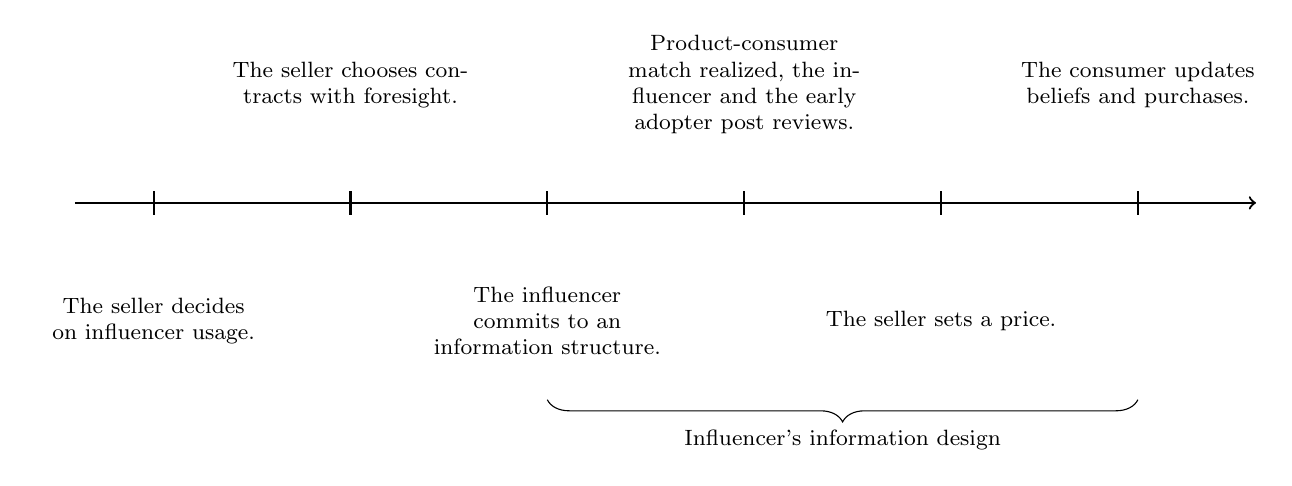
\begin{tikzpicture}[scale=5]
			\footnotesize
			%%%%%%%%%the first line%%%%%%
			%%%%%%%%%%left panel graph*****************
			%\node at (-0.3, 2.45) {$t$};
			\node[align=center,text width=3cm] at (0, 2.2) {The seller decides on influencer usage.};
			
			\node[align=center, text width=3cm] at (0.5, 2.8) {The seller chooses contracts with foresight.};
			
			\node[align=center, text width=3cm] at (1, 2.2) {The influencer commits to an information structure.};
			
			\node[align=center,text width=3cm] at (1.5, 2.8) {Product-consumer match realized, the influencer and the
				early adopter post reviews.};
			\node[align=center,text width=3cm] at (2, 2.2) {
			The seller sets a price.};
			
			\node[align=center,text width=3cm] at (2.5, 2.8) {The consumer updates beliefs and purchases.};
			
			
			\draw [thick, ->] (-0.2,2.5) -- (2.8,2.5);
			\draw [thick] (0,2.47) --(0,2.53);
			\draw [thick] (0.5,2.47) --(0.5,2.53);
			\draw [thick] (1,2.47) --(1,2.53);
			\draw [thick] (1.5,2.47) --(1.5,2.53);
			\draw [thick] (2,2.47) --(2,2.53);
			\draw [thick] (2.5,2.47) --(2.5,2.53);
			
			
			% Add a bracket under timeline between 1 and 7
			\draw[decorate,decoration={brace,amplitude=8pt,mirror}] (1,2) -- (2.5,2) node[midway,below,yshift=-8pt]{Influencer's information design};
			
		\end{tikzpicture}
		\caption{Timeline of the game}
		\label{fig: timeline}
	\end{figure}
	

	
	